 \documentclass[final,3p,times,11pt,onecolumn]{myElsarticle}
\usepackage{float}
\usepackage{times}
\usepackage[utf8]{inputenc}
\usepackage[english]{babel}
\usepackage[T1]{fontenc}
\usepackage{geometry}
\usepackage{color}
\usepackage{soul}
\usepackage{cancel}
\usepackage{subfigure}
\usepackage{enumerate}
\usepackage{amsmath,amsthm,amsfonts,amssymb}
\usepackage{amsthm}
\usepackage{multirow}
\usepackage{graphicx}
\graphicspath{{./figs/}}
\numberwithin{equation}{section}
\usepackage{spverbatim}
\usepackage{fancyhdr}
\usepackage{listings} 
\usepackage{lineno}
\usepackage[none]{hyphenat}
\date{\today}
\setcounter{secnumdepth}{3}
\providecommand{\abs}[1]{\lvert#1\rvert}
\providecommand{\norm}[1]{\lVert#1\rVert}
\setlength\parindent{12pt}		

%\linenumbers

\newcommand{\COM}[1]{{\color{green} #1}}
\newcommand{\HA}[1]{{\color{red} #1}}
\newcommand{\CIP}[1]{{\color{blue} #1}}
\newcommand{\CMV}[1]{{\color{orange} #1}}


\begin{document}

\begin{frontmatter}

%\title{A pressure-velocity coupling strategy based on SIMPLEC: the COMPLEX algorithm}
\title{A SIMPLE-based algorithm with enhanced velocity corrections: the COMPLEX method}
%% A second-neighbour extended correction for segregated p-v coupling algorithms
 
\author[a]{Horacio J. Aguerre}
\author[a,b]{Cesar M. Venier}
\author[b,a]{C\'{e}sar I. Pairetti}
\author[a,c]{Santiago M\'{a}rquez Dami\'{a}n}
\author[a,d]{Norberto M. Nigro}

\address[a]{Centro de Investigación de Métodos Computacionales, CONICET-UNL, Santa Fe, Argentina}
\address[b]{Escuela de Ingeniería Mecánica, Facultad de Ciencias Exactas, Ingeniería y Agrimensura, Universidad Nacional de Rosario, Rosario, Argentina}
\address[c]{Facultad Regional Santa Fe, Universidad Tecnológica Nacional, Santa Fe, Argentina}
\address[d]{Facultad de Ingeniería y Ciencias Hídricas, Universidad Nacional del Litoral, Santa Fe, Argentina}

%Start of abstract
\begin{abstract}
This paper introduces a new pressure-velocity coupling algorithm based on the SIMPLEC method. The new approach considers the neighbour velocity corrections of SIMPLEC as a Taylor series expansion, introducing a first-order term to increase the accuracy of the approximation. The new term includes a velocity gradient which is assumed to be a scalar matrix constrained by means of a mass conservation equation.
The stability of the method is analysed via a Fourier decomposition of the error showing a better convergence rate than SIMPLE and SIMPLEC for high relaxation factors. Afterwards, the new method is tested in two incompressible laminar flow problems where the conclusions of the stability analysis are verified. The current proposal sets a theoretical baseline for further improvements and, in view of the results, it is a promising alternative to improve SIMPLE-based algorithms.
\end{abstract}

\begin{keyword}
SIMPLE algorithm \sep Segregated methods \sep Collocated grids
\sep OpenFOAM(R) \sep Finite Volume Method 
\end{keyword}
\end{frontmatter}

%%%%%%%%%%%%%%%%%%%%%%%%%%%%%%%%%%%%%
\section{Introduction}

A major numerical difficulty for solving the incompressible Navier-Stokes equations arises from the coupling between
the pressure and velocity fields. Several strategies have been proposed to tackle this problem which can
be classified as coupled and segregated methods. The first group solves all the governing
equations at once for all the unknowns \cite{mazhar1, mazhar2, chen, darwish1, darwish2, uroic}. Hence, pressure and velocity are assembled togetherand the non-linearity of the convective term is treated iteratively. Segregated algorithms, in contrast, solve the equations in a sequential fashion for a single variable at a time. The procedure is iterative and ends when the unknowns satisfy a certain convergence criterion \cite{ferziger, versteeg, moukalled}. In general, segregated strategies are superior in terms of memory saving and computational performance but their numerical stability may not be guaranteed when solving strongly-coupled physical problems \cite{wang2, uroic}. Within these group of methods, the penalty method \cite{temam1968methode}, the artificial compression method \cite{harten1977artificial} and projection methods \cite{chorin1, chorin2, temam1968methode} are among the most adopted in CFD codes nowadays \cite{wang2}. In the projection methods, an initial estimation of the velocity is corrected by means of a pressure equation where the velocity field is forced to satisfy the divergence-free condition. In particular, the Fractional Step Methods \cite{kim} rely on a temporal splitting on the velocity where a first estimate is obtained with the momentum equation using an initial guess of the pressure. Then, the remaining velocity contribution is computed by solving a pressure equation based on the mass balance.

Under the scope of the projection methods, a new line of strategies was introduced by Patankar and Spalding with the development of the SIMPLE algorithm \cite{patankar1972}. In this method, a pressure equation is derived after introducing the momentum equation into the mass balance. Then, the velocity field is updated based on the momentum equation including the new values of the pressure field. This procedure is iterative and employs relaxation factors to improve the stability and convergence rate of the method. Focusing on these last aspects, further improvements have been developed taking over the years the SIMPLE algorithm as a starting
point. Among them, the SIMPLER algorithm \cite{patankar1980} enhances the pressure-velocity coupling by solving an additional pressure equation. Another relevant improvement on SIMPLE was proposed by Van Doormal and Raithby \cite{vanDoormal}, who included an approximation of the neighbour velocity corrections to build the pressure equation and the velocity update. This algorithm, called SIMPLEC, suppresses the need for relaxing the pressure field to guarantee stability. In order to solve transient problems, Issa proposed the PISO method \cite{issa,issa2} which consists on including corrector sub-steps to enforce mass conservation without relaxation. Many variants of the SIMPLE method were developed seeking to enhance the robustness and convergence rate of the standard SIMPLE algorithm \cite{tao,qu,cheng2,sun}. Their particular advantages and drawbacks can be found in the literature \cite{moukalled, liu, wang}. Despite the aforementioned efforts to improve SIMPLE-like algorithms, the errors introduced by the decoupling of the variables
cannot be completely eliminated which makes the topic still relevant nowadays \cite{li2017efficient, xiao2018consistent,aoussou2018iterated,aguerre2018oscillation}.

The error introduced by the SIMPLE algorithm comes from neglecting the neighbour velocity to decouple pressure and velocity. 
%If the correction values were known, the discretized system given by the pressure and momentum equations would be equivalent to the original linearized Navier-Stokes problem.
In practice, this approximation requires relaxing the pressure to achieve a stable behaviour towards convergence of the iterative process. Regarding this, the SIMPLEC algorithm considers the neighbour velocity correction equal to the one of the current cell. In other words, it considers the velocity correction as a constant field in the proximity of each cell. This process, in most cases, enhances the ranges of stability avoiding the need to relax the pressure field. The SIMPLEC approximation may be seen as an estimation of the neighbour velocities via a zero-order truncation of a Taylor series expansion. In this context, this work proposes to employ this numerical insight by taking into account a first-order term of the same Taylor series expansion. The approach brings up the need for determining the derivative of the velocity correction, which is a topic of discussion of the present work.

This article is organized as follows. Section 2 describes the SIMPLE and SIMPLEC algorithms and then, in Section 3, the basis and theoretical background of the new method are explained. Subsequently, in Section 4, a stability analysis based on Fourier decomposition is performed for the three mentioned algorithms. Next, in Section 5, a set of laminar flow problems are solved to calibrate and investigate the performance of the new proposal. Finally, a discussion of the results and final comments are presented in the last section.

\section{Theoretical basis of the SIMPLE-based algorithms} \label{sec:theory}

This section presents a general approach for solving the steady-state, incompressible Navier-Stokes equations via segregated pressure-based methods of the SIMPLE familiy. This is done under the framework of the Finite Volume Method (FVM) on collocated grids with the Rhie-Chow correction \cite{rhiechow}. First, the standard SIMPLE algorithm for the pressure and velocity coupling is explained \cite{patankar1972}. Then, the SIMPLEC algorithm is introduced \cite{vanDoormal} following the same formalism and focusing on the approximation of the neighbour velocity corrections \cite{moukalled}. This last aspect is the starting point for the method proposed in this work.

The continuum incompressible Navier-Stokes equations may be written as follows,
\begin{align}
\displaystyle \frac{\partial \boldsymbol{u}}{\partial t} + \nabla \cdotp (\boldsymbol{u} \boldsymbol{u}) &= -\nabla p + \nu\, \Delta \boldsymbol{u} + \boldsymbol{\Phi},
\label{eq:mom1}
\\
\displaystyle \nabla \cdotp \boldsymbol{u} &= 0, 
\label{eq:mass1}
\end{align}
\noindent where $\displaystyle p = (\mathcal{P}/\rho)$, $\rho$ is the mass density field, $\mathcal{P}$ is the pressure field, $\boldsymbol{u}$ is the velocity field, $\nu$ is the kinematic viscosity and $\mathbf{\Phi}$ is a momentum source term.
Based on the FVM and linearizing the convective term, the Eqs.~(\ref{eq:mom1}) and~(\ref{eq:mass1}) may be discretized as:
\begin{align}
a_P\,\boldsymbol{u}_P + \sum_{N} a_{N}\,\boldsymbol{u}_{N} &= b_P\, \boldsymbol{u}^0_P + \boldsymbol{\Phi}_P - \nabla p_P
\qquad \qquad \forall P\,\in\,\Omega,
\label{eq:umom1}
\\
\sum_{f} \boldsymbol{u}_{f} \cdotp \textbf{S}_{f} &= 0
\qquad \qquad \qquad
\qquad \qquad \,\quad \forall P\,\in\,\Omega, 
\label{eq:mass2} 
\end{align}
where the subscript $P$ refers to a given cell of a Finite Volume (FV) mesh $\Omega$, $N$ refers to the values of neighbour cells of $P$ and $f$ refers to values in the faces of the cell $P$, $b_P\, \boldsymbol{u}^0_P$ is the contribution of the previous time-step or iteration and $\textbf{S}_{f}$ is the face-normal vector. Also, $a_P$ and $a_{N}$ are the diagonal and off-diagonal momentum matrix coefficients respectively and the gradient $\nabla p_P$ is computed by linear interpolation of first neighbour values of that field. Further detail can be found in \cite{jasak, moukalled, marquez}.

Eqs.~(\ref{eq:umom1}) and~(\ref{eq:mass2}) are presented in a way that could serve as a starting point for both steady-state and transient algorithm formulations, depending on $a_P$ and $b_P$ definitions \cite{issa2}. For transient solvers, $b_P$ contains the discretized coefficients of the transient term of the momentum equation (e.g. $b_P = V_P/\Delta t$ for first order schemes, being $V_P$ the cell volume and $\Delta t$ the time step) while, for steady-state solvers, it is defined following a numerical relaxation of the momentum equations to enhance the stability of the method \cite{moukalled} (e.g. $b_P = \overline{a}_P\,(1-\omega_u)/\omega_u $, where $\overline{a}_P$ includes the current cell contributions of the advective and diffusive terms and $\omega_u$ is the relaxation coefficient). Therefore, $a_P = \overline{a}_P + V_P/\Delta t$ for transient solvers and $a_P = \overline{a}_P/\omega_u$ for steady-state solvers.  The present work employs on the steady-state formulation.

%The value of $b_P$ is function of the temporal scheme in transient solvers and of the relaxation factor in steady-state solvers, ,  
The system given by Eqs.~(\ref{eq:umom1}) and (\ref{eq:mass2}) may be rewritten in a more suitable way for the subsequent numerical approach. First, the current cell velocity $\boldsymbol{u}_{P}$ may be isolated from Eq.~(\ref{eq:umom1}) as,
\begin{equation}
\label{Eq:UpIsolatedH}
\boldsymbol{u}_P
=
\dfrac
{
\boldsymbol{H}_P
- 
\nabla p_P}
{a_P},
\end{equation}
\noindent where $\boldsymbol{H}_P$ is defined as,
\begin{equation}
\boldsymbol{H}_P
\equiv
-\sum_{N} a_{N}\,\boldsymbol{u}_{N}
+
b_P\, \boldsymbol{u}^0_P 
+ 
\boldsymbol{\Phi}_P.
\end{equation}
Then, Eq.~(\ref{Eq:UpIsolatedH}) is replaced in Eq.~(\ref{eq:mass2}),
\begin{equation}
\sum_{f} 
\left(
\boldsymbol{u}_{P} 
\right)_f
\cdotp 
\textbf{S}_{f} 
=
\sum_{f} 
\left(
\dfrac
{
\boldsymbol{H}_P
- 
\nabla p_P}
{a_P}
\right)_f
\cdotp 
\textbf{S}_{f}
= 
0,
\end{equation}
where the $(\cdot)_f$ operator interpolates cell values to the faces. Finally, an equation for the pressure field is obtained,
\begin{equation}
\label{Eq:firstPressureEq}
\sum_{f} 
\left(
\dfrac
{
\nabla p_P}
{a_P}
\right)_f
\cdotp 
\textbf{S}_{f}
=
\sum_{f} 
\left(
\dfrac
{
\boldsymbol{H}_P
}
{a_P}
\right)_f
\cdotp 
\textbf{S}_{f}.
\end{equation}

Considering that Eqs.~(\ref{Eq:UpIsolatedH}) and (\ref{Eq:firstPressureEq}) must be solved for each cell, there are two linear system of equations: one for the velocity and one for the pressure. Now, for the iterative procedure, a subdivision of the velocity into two contributions is considered,
\begin{align}
\label{Eq:velocitySubdiv}
\boldsymbol{u}_P
= 
\boldsymbol{u}_P^{*} 
+
\boldsymbol{u}_P^{'}, \\
\boldsymbol{u}_N
= 
\boldsymbol{u}_N^{*} 
+
\boldsymbol{u}_N^{'},
\end{align}
where $\boldsymbol{u}^{*}$ is a velocity prediction and $\boldsymbol{u}^{'}$ is the velocity correction. This subdivision leads to an analogous separation of the variable $\boldsymbol{H}_P$,
\begin{equation}
\label{Eq:HSubDivision}
\boldsymbol{H}_P 
=
\boldsymbol{H}_P^{*}
+
\boldsymbol{H}_P^{'},
\end{equation}
where,
\begin{align}
\label{Eq:HStar}
\boldsymbol{H}_P^{*} 
&= -\sum_{N} a_{N}\,\boldsymbol{u}_{N}^{*}
+
b_P\, \boldsymbol{u}^0_P 
+ 
\boldsymbol{\Phi}_P,
\\
\label{Eq:HPrima}
\boldsymbol{H}_P^{'}
&= -\sum_{N} a_{N}\,\boldsymbol{u}_{N}^{'}. 
\end{align}
Considering these last expressions, the iterative procedure begins by computing the momentum balance to predict the velocity $\boldsymbol{u}_P^{*}$ using the previous iteration value of the pressure $p^{0}$,
\begin{equation}
\label{Eq:MomentumPredictor}
\boldsymbol{u}_P^{*}
=
\dfrac
{
\boldsymbol{H}_P^*
- 
\nabla p_P^{0}}
{a_P}.
\end{equation}
After this, the pressure is computed by introducing the Eq.~(\ref{Eq:HSubDivision}) in the mass balance of Eq.~(\ref{Eq:firstPressureEq}),
\begin{equation}
\label{Eq:pressureEqSubdiv}
\sum_{f} 
\left(
\dfrac
{
\nabla p_P}
{a_P}
\right)_f
\cdotp 
\textbf{S}_{f}
=
\sum_{f} 
\left(
\dfrac
{
\boldsymbol{H}_P^{*}
+
\boldsymbol{H}_P^{'}
}
{a_P}
\right)_f
\cdotp 
\textbf{S}_{f}.
\end{equation}

\subsection{The SIMPLE algorithm on collocated grids}

Since the correction velocity values $\boldsymbol{u}_N^{'}$ are not known before solving the pressure equation, an approximation for $\boldsymbol{H}_P^{'}$ must be proposed. In this sense, the SIMPLE method neglects the influence of the neighbour velocity correction which is equivalent to,
\begin{equation}
\label{Eq:simpleAproximation}
\boldsymbol{H}_P^{'} = 0.
\end{equation}
Thus, introducing~Eq.~(\ref{Eq:simpleAproximation}) into (\ref{Eq:pressureEqSubdiv}),
\begin{equation}
\sum_{f} 
\left(
\dfrac
{
\nabla p_P}
{a_P}
\right)_f
\cdotp 
\textbf{S}_{f}
=
\sum_f 
\left(
\dfrac
{
\boldsymbol{H}_P^*
}
{
a_P
}
\right)_f
\cdot
\boldsymbol{S}_f,
\label{eq:div-free5}  
\end{equation}
which is a Poisson problem for the pressure.

In collocated grids, solving this system in a straightforward manner may lead to high-frequency oscillations. The Rhie-Chow correction \cite{rhiechow} seeks to reduce this effect by introducing a stabilizing term, 

\begin{equation}
\label{eq:pEqnSIMPLE2}
\sum_{f} 
\left(
\dfrac
{
\nabla p_P}
{a_P}
\right)_f
\cdotp 
\textbf{S}_{f} 
=
\sum_f 
\left(
\dfrac{
\boldsymbol{H}_P^*
}
{
a_P
}
\right)_f
\cdot
\boldsymbol{S}_f 
+
\sum_f  
\left[
\left(
\frac{\nabla p_P}{a_P}
\right)_f
- 
\left(
\frac{1}{a_P}
\right)_f 
\nabla p_f
\right]
\cdot 
\boldsymbol{S}_f,
\end{equation}
where $\nabla p_f$ is a pressure gradient on a face computed from the pressure values of the adjacent cells. The Eq.~(\ref{eq:pEqnSIMPLE2}) can be rearranged in to obtain the pressure equation as follows,
\begin{equation}\label{eq:pEqnSIMPLE3}
\sum_f \left(\frac{1}{a_P}\right)_f \nabla p_f 
\cdot
\boldsymbol{S}_f 
=  \sum_f \left(\frac{\boldsymbol{H}_P^*}{a_P}\right)_f \cdot \boldsymbol{S}_f.
\end{equation}

To improve the numerical stability of the method, the pressure field is relaxed after Eq.~(\ref{eq:pEqnSIMPLE3}),
\begin{equation}
\label{eq:relaxP}
p_P
=
\omega_P \tilde{p}_P + (1-\omega_P) p_P^0.
\end{equation}
\noindent where $\tilde{p}_P$ is the pressure field obtained from Eq.~(\ref{eq:pEqnSIMPLE3}).

Finally, the velocity value is computed through Eq.~(\ref{Eq:UpIsolatedH}) where the variable $\boldsymbol{H}_P$ is approximated by $\boldsymbol{H}_P^{*}$ (as it was done for the mass balance equation),
\begin{equation}
\label{eq:SIMPLECorr}
\boldsymbol{u}_P
=
\dfrac
{
\boldsymbol{H}_P^*
- 
\nabla p_P}
{a_P}.
\end{equation}
Note that the last equation is explicit since the terms r.h.s. are known. The algorithm continues iteratively from Eq.~(\ref{Eq:MomentumPredictor}), where $\boldsymbol{u}_P^0$ and $p_P^0$ are replaced by the values of $\boldsymbol{u}_P$ and $p_P$ from the previous iteration, until a certain convergence criterion is reached.

% In order to do so, the velocity field $\boldsymbol{u}_P$, originally on cell-centers, needs to be interpolated to the faces obtaining: 
%
% \begin{equation}
% \begin{split}
% \sum_{f} \left( \boldsymbol{H}_P_P - \frac{1}{a_P} \nabla p_P  \right)_f \cdotp \textbf{S}_{f} = 0 
% \end{split}
% \label{eq:pEq1} 
% \end{equation}
%
%Therefore, the Corrector step may be summarized as:
%
%\begin{enumerate}
%
%\item Assemble and solve the pressure based on Eq.~(\ref{eq:pEq1}):
%
%\begin{equation}
%\begin{split}
%\sum_{f} \left( \frac{1}{a_P} \nabla p'_P \right)_f \cdotp \textbf{S}_{f} = \sum_{f} \boldsymbol{u}^*_f \cdotp \textbf{S}_{f}
%\end{split}
%\label{eq:pEq2} 
%\end{equation}


%\CIP{Si conservamos la forma relativa, aquí habría que meter la explicación de Rhie Chow}

%\item {\color{red}Compute} the face fluxes by adding the new pressure contribution:
%
%\begin{equation}
%\begin{split}
%F_f = \boldsymbol{u}^*_f \cdotp \textbf{S}_{f} -  \left( \frac{1}{a_P}\right)_f \nabla p'_f  \cdotp \textbf{S}_{f}
%\end{split}
%\label{eq:Fhat} 
%\end{equation}
%
%\item Correct the cell-centered velocity field based on the new pressure field, using Eq. (\ref{eq:umom3b})
%
%\begin{equation}\label{eq:umom3b}
%\begin{split}
%\boldsymbol{u}_P = \boldsymbol{u}^*_P - \frac{1}{a_P} \nabla p'_P 
%\end{split}
%\end{equation}
%
%\end{enumerate}

%\fi
%Most of the SIMPLE-family algorithms preserve this general structure. In particular, the SIMPLE algorithm \cite{patankar1972}, originally conceived as a steady-state flow solver, adds under-relaxation factors to obtain a stable solution. Another variant is the PISO {\color{red}(Pressure-Implicit with Splitting of Operators)} algorithm, which relies on iterating the Corrector step a given number of times to ensure a correct coupling between pressure and velocity for transient flow problems \cite{issa,issa2}. {\color{red} The SIMPLE-PISO combined technique has been largely adopted in several computational codes (e.g. OpenFOAM(R) \cite{ofpg}) to address transient incompressible flow problems due to its beneficial convergence features. It consists on iterating the corrector steps until a certain mass conservation criterion is fulfilled (as in PISO) and iterating the whole sequence (Momentum Predictor and Corrector Step) several times until both mass and momentum equations are verified for each time step. This algorithm will be adopted in the present work.}

\subsection{Improving the neighbour velocity corrections: the SIMPLEC algorithm}
The SIMPLEC~\cite{vanDoormal} algorithm proposes an approximation for the neighbour velocity correction $\boldsymbol{u}_N'$,
\begin{equation}
\label{Eq:simplecAproximation}
\boldsymbol{u}_N'
=
\boldsymbol{u}_P',
\end{equation}
and therefore the Eq.~(\ref{Eq:HPrima}) may be expressed as,
\begin{equation}
\label{eq:H_SIMPLEC}
\boldsymbol{H}_P'= \left(-\sum_N a_N\right) \boldsymbol{u}'_P.
\end{equation}
This expression may be written in terms of the pressure gradient. To do this, an expression for $\boldsymbol{u}_P^{'}$ is derived by subtracting Eq.~(\ref{Eq:MomentumPredictor}) from Eq.~(\ref{Eq:UpIsolatedH}),
\begin{equation}
\label{Eq:UPrimaIsolated}
\boldsymbol{u}_P'
=
\dfrac
{
\boldsymbol{H}_P'
- 
\left(
\nabla p_P
-
\nabla p_P^{0}
\right)
}
{a_P},
\end{equation}
which, in combination with Eq.~(\ref{eq:H_SIMPLEC}), provides an expression for $\boldsymbol{H}_P'$ as function of the pressure gradient,
\begin{equation}
\label{Eq:HPrima2}
\boldsymbol{H}_P'
= 
\dfrac
{
\left(
\tilde{a}_P
-
a_P
\right)
}
{
\tilde{a}_P
}
\left(
\nabla p_P
-
\nabla p_P^{0}
\right),
\end{equation}
where,
\begin{equation}
\tilde{a}_P
=
a_P + \sum_{N} a_{N}.
\end{equation}
Subsequently, introducing Eq.~(\ref{Eq:HPrima2}) in Eq.~(\ref{Eq:pressureEqSubdiv}),

\begin{equation}
\label{Eq:pressureReplacedSimplec}
\sum_{f} 
\left(
\dfrac
{
\nabla p_P}
{a_P}
\right)_f
\cdotp 
\boldsymbol{S}_{f}
=
\sum_{f} 
\left(
\dfrac
{
\boldsymbol{H}_P^{*}
}
{a_P}
\right)_f
\cdotp 
\boldsymbol{S}_{f}
+
\sum_f
\left[
\dfrac
{
\left(
\tilde{a}_P
-
a_P
\right)
}
{
\tilde{a}_P\,a_P
}
\left(
\nabla p_P
-
\nabla p_P^{0}
\right)
\right]_f
\cdot
\boldsymbol{S}_{f},
\end{equation}
which may be rewritten as,
\begin{equation}
\label{Eq:pressureReplacedSimplec2}
\sum_{f} 
\left(
\dfrac
{
\nabla p_P}
{\tilde{a}_P}
\right)_f
\cdotp 
\boldsymbol{S}_{f}
=
\sum_{f} 
\left(
\dfrac
{
\boldsymbol{H}_P^{*}
}
{a_P}
\right)_f
\cdotp 
\boldsymbol{S}_{f}
+
\sum_f
\left[
\left(
\dfrac{1}
{\tilde{a}_P}
-
\dfrac{1}
{a_P}
\right)
\nabla p^{0}
\right]_f
\cdot
\boldsymbol{S}_f.
\end{equation}
The pressure equation is finally obtained by including an analogous Rhie-Chow correction:

\begin{equation}
\label{eq:pEqnSIMPLEC2}
\begin{array}{ccc}
&
\displaystyle 
\sum_{f} 
\left(
\dfrac
{
\nabla p_P}
{\tilde{a}_P}
\right)_f
\cdotp 
\boldsymbol{S}_{f} 
=
\sum_{f} 
\left(
\dfrac
{
\boldsymbol{H}_P^{*}
}
{a_P}
\right)_f
\cdotp 
\boldsymbol{S}_{f}
+
\sum_f
\left[
\left(
\dfrac{1}
{\tilde{a}_P}
-
\dfrac{1}
{a_P}
\right)
\nabla p^{0}
\right]_f
\cdot
\boldsymbol{S}_f
&
\\
&+& \\
&
\displaystyle 
\sum_f
\left\lbrace
\left(
\dfrac
{
\nabla p
}
{\tilde{a}_P}
\right)_f
-
\left(
\dfrac
{1}
{\tilde{a}_P}
\right)_f
\nabla p_f
+
\left(
\dfrac
{1}
{\tilde{a}_P}
-
\dfrac
{1}
{a_P}
\right)_f
\nabla p^{0}_f
-
\left[
\left(
\dfrac
{1}
{\tilde{a}_P}
-
\dfrac
{1}
{a_P}
\right)
\nabla p^0
\right]_f
\right\rbrace
\cdot
\boldsymbol{S}_f,
&
\end{array}
\end{equation}
which may be simplified as,
\begin{equation}
\sum_f
\left(
\dfrac
{1}
{\tilde{a}_P}
\right)_f
\nabla p_f
\cdot 
\boldsymbol{S}_f
= 
\sum_f 
\left(
\frac{
\boldsymbol{H}_P^*
}{a_P}
\right)_f 
\cdot
\boldsymbol{S}_f
+
\sum_f
\left[
\left(
\dfrac
{1}
{\tilde{a}_P}
-
\dfrac
{1}
{a_P}
\right)_f
\nabla p^{0}_f
\right]
\cdot
\boldsymbol{S}_f.
\label{eq:pEqnSIMPLEC}
\end{equation}

The velocity is computed by including Eq.~(\ref{Eq:HPrima2}) into Eq.~(\ref{Eq:HSubDivision}), and then into Eq.~(\ref{Eq:UpIsolatedH}):

\begin{equation}
\label{eq:uCorrSIMPLEC}
\boldsymbol{u}_P 
=
\dfrac
{
\boldsymbol{H}_P^*
- 
\nabla p_P}
{a_P}
+
\dfrac
{
\left(
\tilde{a}_P
-
a_P
\right)
}
{
\tilde{a}_P\,a_P
}
\left(
\nabla p_P
-
\nabla p_P^{0}
\right).
\end{equation}
where the terms may be reordered to obtain,
\begin{equation}
\label{Eq:velocitySimplec}
\boldsymbol{u}_P 
=
\dfrac
{
\boldsymbol{H}_P^*
- 
\nabla p_P}
{\tilde{a}_P}
+
\left(
\dfrac{1}
{\tilde{a}_P}
-
\dfrac{1}
{a_P}
\right)
\nabla p^{0}.
\end{equation}

In contrast to SIMPLE, SIMPLEC does not relax the pressure since it is not needed to ensure stability. The reader may notice that, if $\tilde{a}_P$ is replaced by $a_P$ in Eqs.~(\ref{eq:pEqnSIMPLEC}) and~(\ref{Eq:velocitySimplec}), SIMPLEC reduces to SIMPLE. 

\section{A COupling Method for Pressure Linked Equations based on series eXpansions: COMPLEX}
\label{sec:COMPLEX}

The approximation of the neighbour velocity corrections of SIMPLEC given by Eq.~(\ref{Eq:simplecAproximation}) can be seen as a zero-order truncation of a Taylor series expansion over $\boldsymbol{u}'_N$. This work proposes to enhance this approximation by preserving first order terms of the same expansion,
\begin{equation}\label{eq:uNTaylor}
\boldsymbol{u}_N' = \boldsymbol{u}_P' + \boldsymbol{x}_{PN}\cdot 
\nabla \boldsymbol{u}_f',
\end{equation}
where $\boldsymbol{x}_{PN}$ is a vector that goes from the cell centroid $P$ to the cell centroid $N$. Thus, $\boldsymbol{H}_P'$ may be written as,
\begin{equation}
\label{Eq:HPrimaComplex}
\boldsymbol{H}_P'
=
\left(
-\sum_N a_N
\right)
\boldsymbol{u}_P' 
+
\left(
-\sum_N a_N
\right)
\left(
\boldsymbol{x}_{PN}\cdot 
\nabla \boldsymbol{u}_f'
\right),
\end{equation}
which combined with Eq.~(\ref{Eq:UPrimaIsolated}) leads to,
\begin{equation}
\label{Eq:HPrimaComplexReady}
\boldsymbol{H}_P'
= 
\dfrac
{
\left(
\tilde{a}_P
-
a_P
\right)
}
{
\tilde{a}_P
}
\left(
\nabla p_P
-
\nabla p_P^{0}
\right)
+
\dfrac{a_P}{\tilde{a}_P}
\,
\boldsymbol{\delta}_P,
\end{equation}
where $\boldsymbol{\delta}_P$ is defined as the second term of the r.h.s. of Eq.~(\ref{Eq:HPrimaComplex}), which will be referred to as the Complex term,
\begin{equation}
\boldsymbol{\delta}_P 
\equiv 
\left(
-\sum_N a_N
\right)
\left(
\boldsymbol{x}_{PN}\cdot 
\nabla \boldsymbol{u}_f'
\right).
\end{equation}
Including Eq.~(\ref{Eq:HPrimaComplexReady}) in Eq.~(\ref{Eq:pressureEqSubdiv}) and following an analogous procedure as done from Eq.~(\ref{Eq:pressureReplacedSimplec}) up to Eq.~(\ref{eq:pEqnSIMPLEC}), the following pressure equation is obtained,
\begin{equation}
\label{Eq:pressureComplex}
\sum_f
\left[
\left(
\dfrac
{1}
{\tilde{a}_P}
\right)_f
\nabla p_f
\right]
\cdot 
\boldsymbol{S}_f
= 
\sum_f 
\left[
\frac{1}{a_P}
\left(
\boldsymbol{H}_P^*
\right)
\right]_f 
\cdot
\boldsymbol{S}_f
+
\sum_f
\left[
\left(
\dfrac
{1}
{\tilde{a}_P}
-
\dfrac
{1}
{a_P}
\right)_f
\nabla p^{0}_f
\right]
\cdot
\boldsymbol{S}_f
+
\sum_f
\left(
\dfrac{\boldsymbol{\delta}_P}{\tilde{a}_P}
\right)_f
\cdot
\boldsymbol{S}_f.
\end{equation}
Then, the velocity is computed including the approximation of Eq.~(\ref{Eq:HPrimaComplex}) in Eq.~(\ref{Eq:HSubDivision}) and~(\ref{Eq:UpIsolatedH}),
\begin{equation}
\label{Eq:velocityComplex}
\boldsymbol{u}_P 
=
\dfrac
{
\boldsymbol{H}_P^*
- 
\nabla p_P}
{\tilde{a}_P}
+
\left(
\dfrac{1}
{\tilde{a}_P}
-
\dfrac{1}
{a_P}
\right)
\nabla p^{0}
+
\dfrac{\boldsymbol{\delta}_P}
{\tilde{a}_P}.
\end{equation}
The Eqs.~(\ref{Eq:pressureComplex}) and (\ref{Eq:velocityComplex}) are similar to Eqs.~(\ref{eq:pEqnSIMPLEC}) and (\ref{Eq:velocitySimplec}) respectively but for the Complex term $\boldsymbol{\delta}_P$. This term requires to define the face gradient $\nabla \boldsymbol{u}_f'$. Putting aside this task, the general structure of the SIMPLEC algorithm remains unaltered. 

\subsection{Computation of the face gradient}
In this work, the face gradient $\nabla \boldsymbol{u}_f' $ is defined as a linear interpolation of a cell-centred gradient $\nabla \boldsymbol{u}_P'$,
\begin{equation}
\label{Eq:UFaceGradient}
\nabla \boldsymbol{u}_f'
=
(\nabla \boldsymbol{u}_P')_f.
\end{equation}
Now, to calculate $\nabla \boldsymbol{u}_P'$, a derivation starts by including the subdivision of the velocity of Eq.~(\ref{Eq:velocitySubdiv}) in the mass balance given by Eq.~(\ref{eq:mass2}),
\begin{equation}
\label{Eq:massEqSubdivided}
\sum_{f} 
\left(
\boldsymbol{u}_{P}^*
+ 
\boldsymbol{u}_{P}'
\right)_f
\cdotp \textbf{S}_{f} 
=
\sum_{f} 
\left(
\boldsymbol{u}_{P}^*
\right)_f
\cdotp \textbf{S}_{f}
+
\sum_{f} 
\left(
\boldsymbol{u}_{P}'
\right)_f
\cdotp \textbf{S}_{f}
=
0
\end{equation}
In this last equation, the face values $\left(\boldsymbol{u}_P'\right)_f$ may be expressed as function of $\nabla \boldsymbol{u}_P'$ by considering the following first-order Taylor expansion,
\begin{equation}
\label{Eq:TaylorOnFace}
\left(
\boldsymbol{u}_P'
\right)_f
=
\boldsymbol{u}_P'
+
\boldsymbol{x}_{Pf}
\cdot 
\nabla \boldsymbol{u}_P'.
\end{equation} 
Now, this may be introduced in Eq.~(\ref{Eq:massEqSubdivided}),
\begin{align}
\sum_f 
\left(
\boldsymbol{u}_P'
+
\boldsymbol{x}_{Pf}
\cdot 
\nabla \boldsymbol{u}_P'
\right)
\cdot 
\boldsymbol{S}_f 
&=
-\sum_f
\left(
\boldsymbol{u}_P^{*}
\right)_{f} 
\cdot 
\boldsymbol{S}_f,
\\
\boldsymbol{u}_P'
\cdot 
\sum_f 
\boldsymbol{S}_f
+
\sum_f 
\left(
\boldsymbol{x}_{Pf}
\cdot 
\nabla \boldsymbol{u}_P'
\right)
\cdot 
\boldsymbol{S}_f,
&=
-\sum_f
\left(
\boldsymbol{u}_P^{*}
\right)_{f} 
\cdot 
\boldsymbol{S}_f
\\
\label{Eq:Last}
\sum_f 
\left(
\boldsymbol{x}_{Pf}
\cdot 
\nabla \boldsymbol{u}_P'
\right)
\cdot 
\boldsymbol{S}_f
&=
-\sum_f
\left(
\boldsymbol{u}_P^{*}
\right)_{f} 
\cdot 
\boldsymbol{S}_f,
\end{align}
where $\sum_f \boldsymbol{S}_f = \boldsymbol{0}$ for convex polyhedra. Then, $\boldsymbol{u}_P^{*}$ is known from Eq.~(\ref{Eq:MomentumPredictor}),
\begin{equation}
\left(
\boldsymbol{u}_P^{*}
\right)_{f}
=
\left[\frac{1}{a_P}\left(\boldsymbol{H}_P^* - \nabla p_P^{0}\right)\right]_f,
\end{equation}
where a similar form of the Rhie-Chow correction term, given in Eq.~(\ref{eq:pEqnSIMPLE2}), is included,
\begin{equation}
\left(
\boldsymbol{u}_P^{*}
\right)_{f}
=
\left[\frac{1}{a_P}\left(\boldsymbol{H}_P^* - \nabla p_P^{0}\right)\right]_f
+
\left[
\left(
\frac{\nabla p_P^{0}}{a_P}
\right)_f
- 
\left(
\frac{1}{a_P}
\right)_f 
\nabla p_f^{0} 
\right],
\end{equation}
leading to, 
\begin{equation}
\left(
\boldsymbol{u}_P^{*}
\right)_{f}
=
 \left(\frac{\boldsymbol{H}_P^*}{a_P}\right)_f 
 -
 \left(\frac{1}{a_P}\right)_f \nabla p_f^{0}.
\end{equation}
Then, replacing this last expression in Eq.~(\ref{Eq:Last}),
\begin{equation}
\label{Eq:mainGradEq}
\sum_f 
\left(
\boldsymbol{x}_{Pf}
\cdot 
\nabla \boldsymbol{u}_P'
\right)
\cdot 
\boldsymbol{S}_f
=
-\sum_f
\left[
\left(\frac{\boldsymbol{H}_P^*}{a_P}\right)_f 
 -
 \left(\frac{1}{a_P}\right)_f \nabla p_f^{0}
 \right]
\cdot 
\boldsymbol{S}_f.
\end{equation}
This last equation relates the cell gradient $\nabla \boldsymbol{u}_P'$ with $\boldsymbol{H}_P^*$ and $\nabla p_f^{0}$, which are known values after the momentum predictor. However, the Eq.~(\ref{Eq:mainGradEq}) is underdetermined since the gradient $\nabla \boldsymbol{u}_P'$ is a second-order tensor with nine scalar unknowns. In order to solve this, an additional approximation is proposed,
\begin{equation}
\nabla \boldsymbol{u}_P'
=
\alpha_P\,
\boldsymbol{I}.
\label{eq:gradApprox}
\end{equation}
This means that the gradient of the velocity corrections is considered to be a scalar matrix. Therefore, it has only one scalar unknown.
Replacing this last definition in Eq.~(\ref{Eq:mainGradEq}),
\begin{align}
\sum_f 
\left(
\boldsymbol{x}_{Pf}
\cdot 
\alpha_P\,
\boldsymbol{I}
\right)
\cdot 
\boldsymbol{S}_f
&=
-\sum_f
\left[
\left(\frac{\boldsymbol{H}_P^*}{a_P}\right)_f 
 -
 \left(\frac{1}{a_P}\right)_f \nabla p_f^{*}
 \right]
\cdot 
\boldsymbol{S}_f,
\\
\alpha_P
\sum_f 
\left(
\boldsymbol{x}_{Pf}
\cdot 
\boldsymbol{I}
\right)
\cdot 
\boldsymbol{S}_f
&=
-\sum_f
\left[
\left(\frac{\boldsymbol{H}_P^*}{a_P}\right)_f 
 -
 \left(\frac{1}{a_P}\right)_f \nabla p_f^{*}
 \right]
\cdot 
\boldsymbol{S}_f,
\end{align}
and, isolating $\alpha_P$,
\begin{equation}
\displaystyle 
\alpha_P
=
\dfrac
{-\displaystyle \sum_f
\left[
\left(\dfrac{\boldsymbol{H}_P^*}{a_P}\right)_f 
 -
 \left(\dfrac{1}{a_P}\right)_f \nabla p_f^{*}
 \right]
\cdot 
\boldsymbol{S}_f}
{\displaystyle\sum_f 
\boldsymbol{x}_{Pf}
\cdot 
\boldsymbol{S}_f}.
\end{equation}
Finally, the face gradient given by Eq.~(\ref{Eq:UFaceGradient}) may be computed using the face interpolated values of $\alpha$,
\begin{equation}
\label{Eq:scalarMatrix}
\nabla \boldsymbol{u}_f'
=
\left(
\alpha_P
\right)_f
\boldsymbol{I}.
\end{equation}

\subsection{Relaxation of the Complex term}
The approximation given in Eq.~(\ref{eq:gradApprox}) provides the mathematical closure of the numerical problem at the cost of reducing the potential of the original proposal. The physical meaning of using a scalar matrix as an estimate of the velocity correction gradient is that it will introduce an isotropic deformation on the fluid. This may not be true once the velocity field is computed with the new pressure values. Taking this into account, a relaxation of the Complex term $\boldsymbol{\delta}_P$ is proposed in order to avoid an overestimation of $\boldsymbol{u}_N'$. In this sense, a relaxation factor is introduced for the Complex term in Eqs.~(\ref{Eq:pressureComplex}) and (\ref{Eq:velocityComplex}), 
\begin{equation}
\label{Eq:pressureComplexRelaxed}
\sum_f
\left[
\left(
\dfrac
{1}
{\tilde{a}_P}
\right)_f
\nabla p_f
\right]
\cdot 
\boldsymbol{S}_f
= 
\sum_f 
\left[
\dfrac{1}{a_P}
\left(
\boldsymbol{H}_P^*
\right)
\right]_f 
\cdot
\boldsymbol{S}_f
+
\sum_f
\left[
\left(
\dfrac
{1}
{\tilde{a}_P}
-
\dfrac
{1}
{a_P}
\right)_f
\nabla p^{0}_f
\right]
\cdot
\boldsymbol{S}_f
+
\kappa
\sum_f
\left(
\dfrac{\boldsymbol{\delta}_P}{\tilde{a}_P}
\right)_f
\cdot
\boldsymbol{S}_f.
\end{equation}
\begin{equation}
\label{Eq:velocityComplexRelaxed}
\boldsymbol{u}_P 
=
\dfrac
{
\boldsymbol{H}_P^*
- 
\nabla p_P}
{\tilde{a}_P}
+
\left(
\dfrac{1}
{\tilde{a}_P}
-
\dfrac{1}
{a_P}
\right)
\nabla p^{0}
+
\kappa
\dfrac{\boldsymbol{\delta}_P}
{\tilde{a}_P}.
\end{equation}
where $\kappa$ is the Complex relaxation factor and its value is between 0 and 1.

\section{Stability Analysis}
\label{sec:fourier}

\subsection{Background of the method}

In order to investigate the numerical stability of the new method, an analysis based on a Fourier decomposition of the error is performed. This technique has proven to be a powerful tool to determine the numerical and physical conditions that guarantee a stable solution for linear equations. Moreover, the methodology is extendable to the analysis of multi-variable discrete systems that are addressed by segregation of the variables. The main feature of this approach is to condense the spatial information into a frequency spectrum where only the term of the frequency that produces the highest amplification of the error is taken into account. In this way, the problem is reduced to the analysis of the Fourier coefficients and its evolution in time \cite{hirsch}. 

On the downside, this technique relies on having constant coefficients in the momentum and pressure equations, which will remain constant until the beginning of the second iteration where $a_P$ and $a_N$ are updated with the new velocity field. That means that a sequence of several SIMPLE iterations cannot be studied via a Fourier decomposition as a whole. Instead, each iteration need to be studied separately. Another issue of the Fourier analysis is that only periodic boundary conditions can be considered for the analysis. Nevertheless, these restrictions are the price to pay to have an analytical tool that gives valuable information about the ranges of stability and error damping of each method as a function of just a few parameters. Moreover, since this technique is used to compare each coupling method under the same conditions, these issues become irrelevant.

Many examples of the usage of this technique can be found in the literature. Shaw et al. \cite{shaw} used it to study the error damping properties of the SIMPLE algorithm in staggered grids. Then, Miller \cite{miller1} extended this analysis to the investigation of the performance of SIMPLE and SIMPLEC on both, collocated and staggered grids. On the other hand, Liu et al. \cite{liu} adopted the same technique to study a large number of algorithms of the SIMPLE family. More recently, Miller et al. \cite{miller2} extended this technique to study Eulerian multiphase flow models, while Venier et al. \cite{venier} studied the stability features of the PISO algorithm for addressing transient and steady-state flow problems.

\subsection{Fourier analysis for SIMPLE-based algorithms}

In this work, a one-dimensional FV discretization is considered to simplify the analysis. A single iteration of the algorithm is studied, which can be separated into three stages: the momentum predictor, the pressure equation and the velocity update. The equations of each stage (for each method) is be written in its Fourier decomposed form. In order to do this, first, these equations are written in terms of the errors of the variables (i.e. pressure and velocity), which are defined as,
\begin{equation}
    e^k_{\phi,M} = \phi^{E}_{M}-\phi_M^{k},
\end{equation}
where $k$ is a given stage of the algorithm ($0$ for the initial values, * for the variables after the momentum predictor, ** for the variables after the pressure equation and *** for the variables after the velocity update), $E$ represents the exact solution of the numerical problem, $\phi$ is a given variable (pressure or velocity) and $M$ represents the spatial location.
% and arrive to some preliminary conclusions about the stability features of the method. Later on, all the methods will be tested in benchmark problems and the stability and convergence rate will be fully assessed.
\begin{figure}[t!]
    \centering
    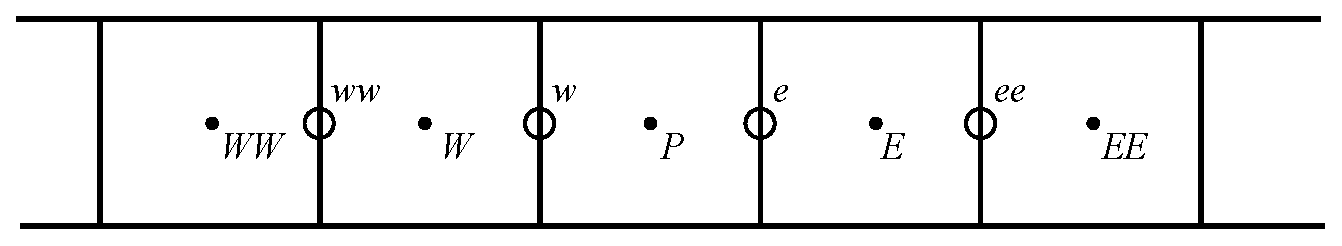
\includegraphics[width=0.7\textwidth]{fig/cells2.eps}
    \caption{One-dimensional FVM discretization.}
    \label{fig:4a}
\end{figure}

First, the momentum predictor, Eq. (\ref{Eq:MomentumPredictor}), is rewritten in terms of the error of the variables as follows,
\begin{equation}
    \dfrac{\overline{a}_P}{\omega_u} \; u_P^* + a_E \; u_E^* + a_W \; u_W^* = \dfrac{1-\omega_u}{\omega_u} \; \overline{a}_P \; u_P^0 - (\nabla p)^0_P + \Phi_P,
\end{equation}
\begin{equation}
    \dfrac{\overline{a}_P}{\omega_u} \; e_{u,P}^* + a_E \; e_{u,E}^* + a_W \; e_{u,W}^* = \dfrac{1-\omega_u}{\omega_u} \; \overline{a}_P \; e_{u,P}^0 - \dfrac{S_f}{2} (e^0_{p,E}-e^0_{p,W}),
    \label{eq:MPerror}
\end{equation}
where $P$, $W$ and $E$ represent the current cell and neighbour cells respectively of the FVM stencil (see Fig. \ref{fig:4a}).
Now, the errors may be written in terms of the Fourier decomposition as,
\begin{equation}
    e^k_{\phi,M} = \alpha^k_{\phi} \; \text{e}^{\left( i \, \theta \, \frac{x_M}{\Delta x}\right)},
    \label{eq:error}
\end{equation}
which, for multivariable systems, become,
\begin{equation}
\begin{bmatrix}
e_u \\
e_p 
\end{bmatrix}^{k}
=
\begin{bmatrix}
u \\
p 
\end{bmatrix}^{E}
-\begin{bmatrix}
u \\
p 
\end{bmatrix}^{k}
=
\begin{bmatrix}
\alpha_u \\
\alpha_p 
\end{bmatrix}^{k}
\; \text{e}^{\left( i \, \theta \, \frac{x_M}{\Delta x}\right)},
\label{eq:fou1}
\end{equation}
where $\Delta x$ represents the distance between the centroids of two adjacent cells.
Replacing each error on Eq.~(\ref{eq:MPerror}) for its corresponding Fourier decomposition, as given by Eq. (\ref{eq:error}), the following equation is obtained:
\begin{equation}
    P_u \; \alpha_u^* = \left( \dfrac{1-\omega_u}{\omega_u} \; \overline{a}_P \right) \; \alpha_u^0 + \left(- \dfrac{S_f}{2} \right) \left(\text{e}^{i \theta} -  \text{e}^{-i \theta} \right) \alpha_p^0,
    \label{eq:MPfou}
\end{equation}
where,
\begin{equation}
P_u = \dfrac{\overline{a}_P}{\omega_u}  + a_E \; \text{e}^{i \theta} + a_W \; \text{e}^{-i \theta}.
\end{equation}
Then, Eq.~(\ref{eq:MPfou}) may be rewritten as,
\begin{equation}
     \alpha_u^* = a_1 \alpha_u^0 + b_1 \alpha_p^0,
    \label{eq:MPfou2}
\end{equation}
where,
\begin{equation}
\begin{split}
     a_1 &= \dfrac{1-\omega_u}{\omega_u} \; \overline{a}_P \; P_u^{-1},
\\
b_1 &= - \left( \dfrac{S_f}{2} \right) \left( \text{e}^{i \theta} -  \text{e}^{-i \theta} \right) \; P_u^{-1},
\end{split}
\end{equation}
and since $p^* = p^0$, the following amplification system is obtained,
\begin{equation}
\begin{bmatrix}
\alpha_u \\
\alpha_p 
\end{bmatrix}^{*} =
[A_1]
\begin{bmatrix}
\alpha_u \\
\alpha_p 
\end{bmatrix}^{0},
\end{equation}
where,
\begin{equation}
A_1 
=
\begin{bmatrix}
a_1 & b_1 \\
0 & 1
\end{bmatrix}. 
\end{equation}
This step of the algorithm, the momentum predictor, is the same for each one of the coupling methods previously described. The next steps, the pressure equation and velocity update, depend on the coupling method, so they are derived separately. First, the SIMPLE algorithm with pressure relaxation is presented, followed by the SIMPLEC and COMPLEX algorithms.

The pressure error equation for SIMPLE is obtained from Eq.~(\ref{eq:pEqnSIMPLE3}), which, in one-dimensional problems, becomes,
\begin{equation}
    S_f \; (e_{p,E}^{**} - 2 e_{p,P}^{**} + e_{p,W}^{**}) = 
     -\left(\dfrac{a_E}{2}\right) (e_{u,EE}^* - e_{u,P}^*) 
    -\left(\dfrac{a_W}{2}\right) (e_{u,P}^* - e_{u,WW}^*)  +
    \left( \dfrac{1-\omega_u}{\omega_u} \right) \left(\dfrac{\overline{a}_P}{2}\right) (e_{u,E}^0 - e_{u,W}^0),
\end{equation}
and the Fourier decomposition of the error (with pressure relaxation) becomes,
\begin{equation}
\begin{split}
    \alpha_p^{**} = &\left( \dfrac{\omega_p}{S_f \Psi} \right) 
                    \left[ \left(-\dfrac{a_E}{2} \right) \left(\text{e}^{2 i \theta} - 1 \right) +
                            \left(-\dfrac{a_W}{2} \right) \left(1 - \text{e}^{-2 i \theta}\right)
                    \right] \alpha_u^{*}, \\
                    & + \left( \dfrac{\omega_p}{S_f \Psi} \right) 
                    \left[ \left(\dfrac{1-\omega}{\omega} \right) \left(\dfrac{\overline{a}_P}{2} \right) \left(\text{e}^{i \theta} - \text{e}^{- i \theta} \right) 
                    \right] \alpha_u^{0}, \\
                    & + (1-\omega_p) \; \alpha_p^*,   
\end{split}
\end{equation}

\noindent where $\alpha_u^{**} = \alpha_u^{*}$ and,

\begin{equation}
    \Psi = \text{e}^{i \theta} - 2 + \text{e}^{- i \theta}.
\end{equation}

For the velocity update, Eq.~(\ref{eq:SIMPLECorr}), the equation for the error may be written as,

\begin{equation}
    e_{u,P}^{***} = -\dfrac{\omega_u a_E}{\overline{a}_P} e_{u,E}^{*} -\dfrac{\omega_u a_W}{\overline{a}_P} e_{u,W}^{*} +
                   -\dfrac{\omega_u S_f}{2 \overline{a}_P} (e_{p,E}^{**}-e_{p,W}^{**}) +
                   (1-\omega_u) \; e_{u,P}^0,
\end{equation}
which, in Fourier terms, becomes,

\begin{equation}
    \alpha_{u}^{***} = \left[\left(-\dfrac{\omega_u a_E}{\overline{a}_P}\right) \text{e}^{i \theta} + \left(- \dfrac{\omega_u a_W}{\overline{a}_P}\right) \text{e}^{- i \theta}\right] \alpha_u^{**} +
                   \left[\left(-\dfrac{\omega_u S_f}{2 \overline{a}_P}\right) \left(\text{e}^{i \theta}-\text{e}^{-i \theta}\right) \right] \alpha_p^{**} +
                   (1-\omega_u) \; \alpha_u^0,
\end{equation}
with $\alpha_p^{***}=\alpha_p^{**}$.
Finally, the amplification of the sequence when adding the pressure equation is,

\begin{equation}
\begin{bmatrix}
\alpha_u \\
\alpha_p 
\end{bmatrix}^{**} =
[A^S_2]
\begin{bmatrix}
\alpha_u \\
\alpha_p 
\end{bmatrix}^{*} +
[A^S_4]
\begin{bmatrix}
\alpha_u \\
\alpha_p 
\end{bmatrix}^{0} =
([A^S_2] [A_1] + [A^S_4])
\begin{bmatrix}
\alpha_u \\
\alpha_p 
\end{bmatrix}^{0},
\end{equation}
and, adding the velocity update amplification contribution, the total amplification matrix ($A^S$) for the SIMPLE algorithm is given by,

\begin{equation}
\begin{bmatrix}
\alpha_u \\
\alpha_p 
\end{bmatrix}^{***} =
[A^S_3]
\begin{bmatrix}
\alpha_u \\
\alpha_p 
\end{bmatrix}^{**} +
[A^S_5]
\begin{bmatrix}
\alpha_u \\
\alpha_p 
\end{bmatrix}^{0} =
([A^S_3] [A^S_2] [A_1] + [A^S_3] [A^S_4] + [A^S_5])
\begin{bmatrix}
\alpha_u \\
\alpha_p 
\end{bmatrix}^{0} =
[A^S]
\begin{bmatrix}
\alpha_u \\
\alpha_p 
\end{bmatrix}^{0},
\end{equation}
where,
\begin{equation}
[A^S_2]= 
\begin{bmatrix}
1 & 0 \\
c^S_2 & d^S_2
\end{bmatrix}
\; \; \; \; \; \;
[A^S_3]= 
\begin{bmatrix}
a^S_3 & b^S_3 \\
0 & 1
\end{bmatrix}
\; \; \; \; \; \;
[A^S_4]= 
\begin{bmatrix}
0 & 0 \\
c^S_4 & 0
\end{bmatrix}
\; \; \; \; \; \;
[A^S_5]= 
\begin{bmatrix}
a^S_5 & 0 \\
0 & 0
\end{bmatrix},
\end{equation}
and,
\begin{equation}
\begin{split}
     c^S_2 &= \left( \dfrac{\omega_p}{S_f \Psi} \right) 
                    \left[ \left(-\dfrac{a_E}{2} \right) \left(\text{e}^{2 i \theta} - 1 \right) +
                            \left(-\dfrac{a_W}{2} \right) \left(1 - \text{e}^{-2 i \theta}\right)
                    \right], \\
     d^S_2 &= (1-\omega_p), \\
     a^S_3 &= \left(-\dfrac{\omega_u a_E}{\overline{a}_P}\right) \text{e}^{i \theta} + \left(- \dfrac{\omega_u a_W}{\overline{a}_P}\right) \text{e}^{- i \theta}, \\
     b^S_3 &= \left(-\dfrac{\omega_u S_f}{2 \overline{a}_P}\right) \left(\text{e}^{i \theta}-\text{e}^{-i \theta}\right), \\ 
     c^S_4 &= \left( \dfrac{\omega_p}{S_f \Psi} \right) 
                     \left(\dfrac{1-\omega_u}{\omega_u} \right) \left(\dfrac{\overline{a}_P}{2} \right) \left(\text{e}^{i \theta} - \text{e}^{- i \theta} \right),  \\
     a^S_5 &= (1-\omega_u).     
\end{split}
\end{equation}

For each method, the total amplification matrix is defined as the product of the matrices of each step following the next rule,
\begin{equation}
[A^m] = ([A^m_3] [A^m_2] [A_1] + [A^m_3] [A^m_4] + [A^m_5]),
\end{equation}
where the superscript $m$ indicates the coupling method being considered ($S$ for SIMPLE, $C$ for SIMPLEC and $X$ for COMPLEX).

Looking at Eqs.~(\ref{eq:pEqnSIMPLEC2}) and~(\ref{eq:uCorrSIMPLEC}), and taking into account the relation between $\nabla p_P^*$ and the velocity field after the momentum predictor given by Eq. (\ref{Eq:MomentumPredictor}), the amplification of the error for the pressure equation and the velocity update of SIMPLEC have a few differences compared to the SIMPLE amplification matrices,

\begin{equation}
\begin{split}
     c^C_2 &= c_2^S + \left(\dfrac{a_E + a_W}{2}\right) (\text{e}^{i    \theta} - \text{e}^{-i \theta}), \\
     d^C_2 &= 1, \\
     a^C_3 &= \left(\dfrac{\overline{a}_P}{\omega_u \; \tilde{a}_P}\right) a_3^S + \dfrac{a_E+a_W}{\tilde{a}_P}, \\
     b^C_3 &= \left(\dfrac{\overline{a}_P}{\omega_u \; \tilde{a}_P}\right) b_3^S, \\ 
     c^C_4 &= \dfrac{1}{\omega_p} c^S_4, \\
     a^C_5 &= \left(\dfrac{\overline{a}_P}{\omega_u \; \tilde{a}_P}\right) a^S_5. 
\end{split}
\end{equation}

The same procedure may be applied to the COMPLEX method based on Eqs. (\ref{Eq:pressureComplexRelaxed}) and (\ref{Eq:velocityComplexRelaxed}). Here, it should be noticed that defining the gradient of the velocity correction $\nabla \boldsymbol{u}_P'$ using a single scalar unknown $\alpha$, is no longer an approximation for one-dimensional problems. Eq. (\ref{eq:gradApprox}) now provides mathematical closure for the problem without the need for any assumption, since the gradient of a vector field in one-dimensional problems is, in fact, a scalar value. The amplification matrix elements for COMPLEX now become,

\begin{equation}
\begin{split}
     c^X_2 = c_2^C &+ \left(\dfrac{a_E}{8}\right) \left(\text{e}^{3 i \theta} + \text{e}^{2 i \theta} - 2 \text{e}^{i \theta} - 2 + \text{e}^{-i \theta} + \text{e}^{-2 i \theta}\right) + \left(-\dfrac{a_W}{8}\right) \left(\text{e}^{2 i \theta} + \text{e}^{i \theta} - 2 - 2 \text{e}^{-i \theta} + \text{e}^{-2 i \theta} + \text{e}^{-3 i \theta}\right), \\
     d^X_2 = d^C_2,& \\
     a^X_3 = a^C_3 &+ \left(\dfrac{a_E}{4}\right) \left(\text{e}^{2 i \theta} + \text{e}^{i \theta} - 1 - \text{e}^{-i \theta} \right) + \left(-\dfrac{a_W}{4}\right) \left(\text{e}^{i \theta} + 1 - \text{e}^{- i \theta} - \text{e}^{-2 i \theta} \right), \\
     b^X_3 = b_3^C,& \\ 
     c^X_4 = c^C_4,& \\
     a^X_5 = a^C_5.&     
\end{split}
\end{equation}

The von Neumann stability criterion \cite{hirsch} is applied to determine the range of stability of each method. For multivariable problems, this criterion may be expressed as,

\begin{equation}
\beta(\theta) = \text{max}_i \{ |\lambda_i(\theta)| \} \leq 1
\label{eq:AmpCrit}
\end{equation}

\noindent where $\beta$ is the amplification factor and $\lambda_i$ are the eigenvalues of the amplification matrix $[A^m]$. If Eq. (\ref{eq:AmpCrit}) is verified for each frequency, then the method will be considered numerically stable (under the hypothesis of the Fourier analysis). Moreover, the value of $\beta$ gives a notion about the error damping or convergence rate of the method. If the values are below but close to unity, then the method will have a slow convergence rate, while the opposite happens when the values are close to zero.

\subsection{Results}
The von Neumann stability criterion is evaluated for the different methods studied in this work. Fig.~\ref{fig:1a} shows the amplification factor for each method for low and high mesh-Reynolds numbers, ($Re_h = \Delta x\, U/\nu$), and using the following relaxation factors: $\omega_u=0.7$, $\omega_p = 1$ for SIMPLEC and COMPLEX, and $\omega_p=1-\omega_u$ for SIMPLE.  It is observed that SIMPLE has a higher amplification factor (slower convergance rate) for each frequency and for each $Re_h$ considered. On the other hand, the SIMPLEC method gets slightly affected with the change of $Re_h$ while COMPLEX does not show any significant variation. All methods show a stable behavior under the Fourier conditions, while COMPLEX and SIMPLEC show lower amplification factors than those of SIMPLE.
\begin{figure}[t!!]
    \centering
    \includegraphics[width=\textwidth]{fig/Re_fourier.pdf}
    \caption{Amplification factor for $Re_h=0.001$ (left) and $Re_h=1000$ (right)}
    \label{fig:1a}
\end{figure}
Fig.~\ref{fig:1b} shows the sensitivity of the amplification factor to the momentum relaxation factor for all frequencies and for the three coupling methods. The results are obtained for a $Re_h=1$ and always considering the rule $\omega_P = 1 - \omega$ for SIMPLE. While the SIMPLE algorithm does not show any significant improvement for higher values of $\omega$ (even showing a range of instability for low frequencies at $\omega_u=0.95$ and $\omega_P=0.05$), the SIMPLEC algorithm shows a depletion in its performance for high momentum relaxation factors (tending to unity for $\theta=0$ as $\omega_u$ tends to 1). In this aspect, the COMPLEX algorithm shows a clear advantage over the other two methods by preserving the overall error damping, even for high momentum relaxation factors.     
\begin{figure}[t!!]
    \centering
    \includegraphics[width=\textwidth]{fig/w_fourier.pdf}
    \caption{Amplification factor for $\omega_u=0.7$ (left) and $\omega_u=0.95$ (right)}
    \label{fig:1b}
\end{figure}    
This theoretical advantage is very important since it indicates that the good performance of the method holds up even when the convergence rate to the steady-state solution is accelerated by increasing the momentum relaxation factors. 

The analysis is deepened by considering a continuous range of relaxation factors from $0$ to $1$ for the three methods, as shown in Fig. \ref{fig:1c}. These figures show a clear advantage of SIMPLEC over SIMPLE for almost every relaxation factor considered, and a clear advantage of COMPLEX over SIMPLEC for high values of the amplification factor. Here it may be noted that, for very low values of $\omega_u$, all methods tend to the same stability behavior.
\begin{figure}[b!]
    \centering
    \includegraphics[width=\textwidth]{fig/maps_fourier.pdf}
    \caption{Amplification values for SIMPLE (a), SIMPLEC (b) and COMPLEX (c) for different relaxation factors and frequencies}
    \label{fig:1c}
\end{figure}    
    
To quantify the overall error damping for a general problem, where the initial solution is formed by an equally distributed amount of modes (i.e. assuming that there is no frequency that is clearly dominant over the others in the initial values of $u$ and $p$ fields), frequency-average amplification factor is considered. This is shown in Fig.~\ref{fig:1d}, where the mean value of $\beta$ over all frequencies is plotted for all the possible values of the momentum relaxation factor. Here it is also clear that, while all methods are stable under these conditions, the SIMPLEC and COMPLEX algorithms are clearly more efficient in terms of the error damping, and the COMPLEX algorithm outperforms SIMPLEC when the relaxation factor is increased. 

\begin{figure}[t!]
    \centering
    \includegraphics[width=0.5\textwidth]{fig/meanAmp.pdf}
    \caption{Mean amplification factor as a function of the momentum relaxation factor $\omega_u$}
    \label{fig:1d}
\end{figure}  

\section{Test cases}
\label{sec:cases}

In this section, the COMPLEX method is analysed in incompressible, laminar and stationary Newtonian flow problems. The numerical performance of the method is compared with SIMPLE and SIMPLEC by measuring the total number of iterations required to achieve a convergence criterion. The details of each problem are explained followed by the definition of the convergence criterion adopted. Two different analysis over the COMPLEX method are performed: first, a series of simulations are carried out to investigate the Complex factor $\kappa$, and then, a comparison of the current proposal with SIMPLE and SIMPLEC is presented for various conditions. 

\subsection{Problems description}\label{Section:problemDescription}
 The evaluation of the COMPLEX method is performed by solving two tests for incompressible and stationary flows. The first of them is a cubic cavity test and the second one is a Backward Facing Step (BFS) channel.

All the simulations use the same numerical setup. The convective terms are discretised with an upwind scheme and the pressure gradient operator is computed with a Gauss-based formula using linear interpolation to define the face values. The diffusive terms are discretised with a Gauss-based formula where the face gradient is assembled with a first-neighbour stencil. The linear system of equations are solved until the residuals for both momentum and mass balances decrease two orders of magnitude. The momentum relaxation factor $\omega_u$ is a variable of the parametric study. The pressure relaxation factor $\omega_p = 1$ for COMPLEX and SIMPLEC, while for SIMPLE is defined as $\omega_p = 1 - \omega_u$.

\subsubsection{Cubic cavity}
 A graphical scheme of this problem is depicted in Fig.~\ref{Fig:Cavity}.
\begin{figure}[t!!!]
\centering
\includegraphics[width=5cm]{fig/Cases/Cavity.pdf}
\caption{The cubic cavity problem where a fixed tangential velocity is imposed on the upper face.}
\label{Fig:Cavity}
\end{figure} 
Here, a tangential fixed velocity of 1 m/s is imposed on the upper face of the cubic domain of length 1 m. The remaining faces of the cavity are walls with a non-slip condition. The case is solved using two different values of the kinematic viscosity, $\nu = 2.5 \times 10^{-3}$ m$^2$/s ($Re=400$) and $\nu = 2.5$ m$^2$/s ($Re=0.4$). For the purposes of this work, the cavity is discretised with hexahedral cells using three different refinement levels: a coarse mesh with 25 divisions per side (15625 cells), a medium mesh with 50 divisions per side ($1.25 \times 10^{5}$ cells) and a fine mesh with 100 divisions per side ($10^{6}$ cells).

\subsubsection{Backward Facing Step}
The domain and dimensions of this test are shown in Fig.~\ref{Fig:Geometria3}.
\begin{figure}[t!!!]
\centering
\includegraphics[width=12cm]{fig/Cases/Geometria3.pdf}
\caption{Description of the BFS domain where its dimensions are defined relative to the inlet height $h = 1$ m.}
\label{Fig:Geometria3}
\end{figure}
At the inlet, a constant normal velocity of 1 m/s is imposed. The outlet has a constant pressure and the remaining faces of the channel are walls with a non-slip condition. Analogously to the cavity case, the problem is simulated with two different viscosity values, $\nu = 5.141 \times 10^{-3}$ m$^2$/s ($Re=389$) and $\nu = 5.141$ m$^2$/s ($Re=0.389$). The domain is discretized with hexahedral cells using three different mesh sizes as defined in Table~\ref{Table:BFSMeshes} with a variable cell size as shown in Fig.~\ref{Fig:Factores}, where the regions near the wall and the step are more refined than the rest of the domain.
\begin{table}[b!]
\centering
\begin{tabular}{cccccccc}
\hline 
\multirow{2}{1cm}{Mesh Level} & \multicolumn{3}{c}{Pre-step divisions} & \multicolumn{3}{c}{Post-step divisions} & \multirow{2}{1cm}{Total Cells} \\ 
\cline{2-7} 
&  $x-$axis &  $y-$axis &  $z-$axis &  $x-$axis &  $y-$axis &  $z-$axis \\ 
\hline 
Coarse & 20 & 40 & 8 & 26 & 40 & 16 & 23040 \\ 
Medium & 40 & 80 & 15 & 52 & 80 & 30 & 172800 \\ 
Fine & 80 & 160 & 30 & 104 & 160 & 60 & 1382400 \\ 
\hline 
\end{tabular}
\caption{Scheme of divisions for the BFS case. The pre-step and post-step are the upstream and downstream regions of the step transversal section.}
\label{Table:BFSMeshes}
\end{table}

\begin{figure}[b!!!]
\centering
\includegraphics[width=16cm]{fig/Cases/Factores.pdf}
\caption{Variable cell refinement in the BFS.  On the left figure, the cell size grows from the step point up to the inlet and outlet boundaries and from the lateral walls up to the middle longitudinal section. On the right, the cell size in the post-step regions grows from the bottom and upper walls up to the middle height section of the channel.}
\label{Fig:Factores}
\end{figure}

\subsection{Error measurement}
To analyse the rate of convergence of the different algorithms, an error norm is defined. This norm is the residual field of the discretized Navier-Stokes equations, which are computed for each cell $P$ of the FV mesh $\Omega$. Then, the momentum residual is expressed as,
\begin{equation}
\label{Eq:R1Discretized}
R_1(P)
=
a_P\,\boldsymbol{u}_P + \sum_{N} a_{N}\,\boldsymbol{u}_{N} 
-b_P\, \boldsymbol{u}^0_P - \boldsymbol{\Phi}_P + \nabla p_P
\qquad \qquad \forall P\,\in\,\Omega,
\end{equation}
and, analogously, the mass residual is computed as follows,
\begin{equation}
R_2(P)
=
\sum_f
\boldsymbol{u}_f
\cdot
\boldsymbol{S}_f
\qquad \qquad
\forall P\,\in\,\Omega,
\end{equation}
where the face velocity value $\boldsymbol{u}_f$ is replaced in terms of the momentum equation as it was done in Eq.~(\ref{Eq:firstPressureEq}),
\begin{equation}
\label{Eq:R2Discretized}
R_2(P)
=
\sum_f 
\left(
\frac{1}{a_P}
\right)_f 
\nabla p_f
\cdot
\boldsymbol{S}_f 
-
\sum_f
\left(
\frac{\boldsymbol{H}_P}
{a_P}
\right)_f 
\cdot 
\boldsymbol{S}_f
\qquad \qquad
\forall P\,\in\,\Omega.
\end{equation}
Then, the Root Mean Square (RMS) of the $R_1$ and $R_2$ fields are computed, 
\begin{align}
\overline{R}_1
&=
\sqrt
{
\sum_{P\,\in\,\Omega}
R_1(P)^2
},
\\
\overline{R}_2
&=
\sqrt
{
\sum_{P\,\in\,\Omega}
R_2(P)^2
}.
\end{align}
Regarding $\overline{R}_1$ and $\overline{R}_2$, the following convergence criterion is proposed: a numerical simulation will be considered converged if both values, $\overline{R}_1$ and $\overline{R}_2$  are below a tolerance of $10^{-9}$,
\begin{equation}
\label{Eq:convergencecriterion}
\left\lbrace
\begin{array}{c}
\overline{R}_1 \leq 10^{-9} \\
\overline{R}_2 \leq 10^{-9}
\end{array}
\right..
\end{equation}

It is important to highlight that the residuals are only function of the velocity, pressure, and of the momentum equation coefficients which are equally assembled for the three methods studied. Thus, the computation of $\overline{R}_1$ and $\overline{R}_2$ are independent of the coupling method. 

\subsection{Study of the Complex factor $\kappa$}
In this section, the influence of $\kappa$ on the convergence rate is analysed in combination with the relaxation factor for the momentum equation $\omega_{u}$ measuring the number of iterations to reach convergence as defined in Eq.~(\ref{Eq:convergencecriterion}). Here, a series of simulations of the cavity and BFS problems are solved using the medium refinement level. For each case, two different physical configurations are addressed according to the proposed Reynolds numbers. Each one of the four simulations are solved varying the values of $\kappa$ and $\omega_{u}$. The Complex factor ranges from 0 to 1 with a step of $0.05$ (21 values) and the relaxation factor ranging from 0.8 up to 1 with a step of $0.1$ (21 values). Altogether, this parametric study consists of 1764 simulations.

In order to compare the performance of the methods, the relative number of iterations ($RI$) is defined as follows, 
\begin{equation}
\label{Eq:relativeIndex}
RI(\omega_u, \kappa)
=
\dfrac
{
NI(\omega_u, \kappa) - NI(\omega_u, 0)
}
{
NI(\omega_u, 0)
}
\times
100 \%,
\end{equation}
where $NI(\omega_u, \kappa)$ is the number of iterations required for convergence using the relaxation value $\omega_u$ and the Complex factor $\kappa$. In this context, $NI(\omega_u, 0)$ is equivalent to the number of iterations required for convergence of the SIMPLEC algorithm. Fig.~\ref{Fig:FactorLowRe} shows $RI$ values for all the studied cases.

The results of the simulations are presented in the Tables~\ref{Table:Cavity_LowRe}, \ref{Table:BFS_LowRe}, \ref{Table:Cavity_HighRe} and \ref{Table:BFS_HighRe}, and in Fig.~\ref{Fig:FactorLowRe}. Here, the required number of iterations to reach the convergence as function of $\omega_u$ and $\kappa$ is shown. The tables focus on the results that are closer to the optimal values of $\omega_u$ (between 0.92 and 1) using a $\kappa$ step of 0.1 instead of 0.05. 
 
The Tables~\ref{Table:Cavity_LowRe},~\ref{Table:BFS_LowRe}, and the upper plots of Fig.~\ref{Fig:FactorLowRe} present the results for relative low Reynolds simulations, while Tables~\ref{Table:Cavity_HighRe},~\ref{Table:BFS_HighRe}, and the lower plots of Fig.~\ref{Fig:FactorLowRe} present the results for relative high Reynolds simulations. 

In general, it is concluded that the addition of the Complex term does not influence the convergence when using low relaxation factors. On the contrary, with high values of $\omega_u$, the addition of the Complex term reduces the number of iterations to approximately 20 $\%$. The best results are obtained with values of the Complex factor $\kappa \leq 0.5$, while $\kappa \geq 0.5$ values may induce instabilities. In particular, the BFS problem at Re = 389 presents an extended divergence zone for the highest values of $\omega_u$, followed by a slow convergence zone (coloured in grey) for lower values of $\omega_u$. Despite this behaviour, the simulations are stable and have a maximum convergence rate for low values of $\kappa$.
\begin{table}[b!!]
\centering
\begin{tabular}{c|ccccccccccc}
\hline 
$\omega_u\,\backslash\:\kappa$ & 0 & 0.1 & 0.2 & 0.3 & 0.4 & 0.5 & 0.6 & 0.7 & 0.8 & 0.9 & 1 \\ 
\hline 
1 & div & div & div & div & div & div & div & div & div & div & div \\ 
0.99 & 1993 & 1702 & 1742 & 1754 & 1747 & 1742 & 1761 & div & div & div & div \\ 
0.98 & 991 & 842  & 845 & 856 & 866 & 870 & 870 & 868 & 865 & 863 & 864 \\ 
0.97 & 658 & 551  & 559 & 560 & 565 & 570 & 574 & 575 & 575 & 575 & 573 \\ 
0.96 & 491 &425  & 414 & 416 & 418 & 421 & 424 & 426 & 427 & 428 & 428 \\ 
0.95 & 391 & 348 & 327 & 330 & 332 & 333 & 335 & 337 & 338 & 339 & 339 \\ 
0.94 & 373 & 373 & 373 & 373 & 373 & 373 & 373 & 373 & 373 & 373 & 373 \\ 
0.93 & 438 & 438 & 438 & 438 & 438 & 438 & 438 & 438 & 438 & 438 & 438 \\ 
0.92 & 504 & 504 & 504 & 504 & 504 & 504 & 504 & 504 & 504 & 504 & 504 \\ 
\hline 
\end{tabular} 
\caption{Required number of iterations at convergence for the Cavity case with Re = $0.4$}
\label{Table:Cavity_LowRe}
\end{table}
\begin{table}[b!!]
\centering
\begin{tabular}{c|ccccccccccc}
\hline 
$\omega_u\,\backslash\:\kappa$ & 0 & 0.1 & 0.2 & 0.3 & 0.4 & 0.5 & 0.6 & 0.7 & 0.8 & 0.9 & 1 \\ 
\hline 
1 & div & div & div & div & div & div & div & div & div & div & div \\ 
0.99 & 1974 & 1697 & 1753 & 1865 & 1941 & 1993 & div & div & div & div & div \\ 
0.98 & 981 & 816 & 844 & 854 & 874 & 904 & 929 & 949 & 966 & 980 & 992 \\ 
0.97 & 651 & 528 & 550 & 560 & 565 & 571 & 581 & 594 & 606 & 618 & 627 \\ 
0.96 & 486 & 392 & 403 & 413 & 418 & 421 & 424 & 428 & 435 & 442 & 449 \\ 
0.95 & 387 & 320 & 317 & 324 & 330 & 333 & 335 & 336 & 339 & 342 & 346 \\ 
0.94 & 320 & 272 & 259 & 266 & 271 & 274 & 276 & 277 & 278 & 280 & 282 \\ 
0.93 & 273 & 237 & 220 & 225 & 229 & 232 & 234 & 235 & 236 & 237 & 238 \\ 
0.92 & 240 & 233 & 233 & 233 & 233 & 233 & 233 & 233 & 233 & 233 & 233 \\ 
\hline 
\end{tabular}
\caption{Required number of iterations at convergence for the BFS case with Re = 0.389}
\label{Table:BFS_LowRe}
\end{table}
\begin{table}[t!!]
\centering
\begin{tabular}{c|ccccccccccc}
\hline 
$\omega_u\,\backslash\:\kappa$ & 0 & 0.1 & 0.2 & 0.3 & 0.4 & 0.5 & 0.6 & 0.7 & 0.8 & 0.9 & 1 \\ 
\hline 
1 & div & div & div & div & div & div & div & div & div & div & div \\ 
0.99 & 1611 & 1321 & 1286 & 1333 & 1357 & div & div & div & div & div & div \\ 
0.98 & 802 & 693 & 652 & 635 & 648 & 662 & 671 & 678 & 682 & div & div \\ 
0.97 & 532 & 471 & 448 & 431 & 423 & 427 & 435 & 441 & 446 & 449 & 452 \\ 
0.96 & 398 & 357 & 342 & 330 & 321 & 317 & 319 & 323 & 327 & 331 & 333 \\ 
0.95 & 318 & 288 & 277 & 269 & 262 & 257 & 255 & 256 & 258 & 261 & 263 \\ 
0.94 & 266 & 243 & 235 & 229 & 225 & 221 & 218 & 216 & 215 & 216 & 217 \\ 
0.93 & 239 & 225 & 218 & 214 & 211 & 211 & 211 & 210 & 210 & 210 & 209 \\ 
0.92 & 243 & 243 & 242 & 242 & 242 & 241 & 241 & 241 & 241 & 241 & 240 \\ 
\hline 
\end{tabular}
\caption{Required number of iterations at convergence for the Cavity case with Re = 400}
\label{Table:Cavity_HighRe}
\end{table}
\begin{table}[t!!]
\centering
\begin{tabular}{c|ccccccccccc}
\hline 
$\omega_u\,\backslash\:\kappa$ & 0 & 0.1 & 0.2 & 0.3 & 0.4 & 0.5 & 0.6 & 0.7 & 0.8 & 0.9 & 1 \\ 
\hline 
1 & div & div & div & div & div & div & div & div & div & div & div \\ 
0.99 & div & div & div & div & div & div & div & div & div & div & div \\ 
0.98 & 818 & 624 & 632 & 637 & div & div & div & div & div & div & div \\ 
0.97 & 540 & 427 & 422 & 428 & 435 & div & div & div & div & div & div \\ 
0.96 & 403 & 329 & 323 & 327 & 329 & 478 & 3086 & div & div & div & div \\ 
0.95 & 322 & 272 & 264 & 266 & 268 & 351 & 712 & 4714 & div & div & div \\ 
0.94 & 269 & 236 & 227 & 226 & 250 & 320 & 483 & 1151 & div & div & div \\ 
0.93 & 240 & 225 & 218 & 221 & 246 & 299 & 397 & 608 & 1427 & div & div \\ 
0.92 & 242 & 235 & 230 & 232 & 256 & 292 & 351 & 457 & 696 & 1087 & 8863 \\ 
\hline 
\end{tabular}
\caption{Required number of iterations at convergence for the BFS case with Re = 389}
\label{Table:BFS_HighRe}
\end{table}
\begin{figure}[t!!!!!!!]
\centering
\includegraphics[width=17cm]{fig/Results/FactorLowRe.pdf}
\caption{Isolines of RI as function of the momentum relaxation factor, the Complex factor for the Cavity and BFS cases, and the values of the Reynolds number employed respectively.}
\label{Fig:FactorLowRe}
\end{figure}

In view of these results, a Complex factor $\kappa = 0.2$ will be used in the following analysis since it is adequate to speed up the convergence without losing stability. % This last inference is determined based on two different numerical problems (Cavity and BFS) in the range of Reynolds number between $0.4$ and $400$. 

 
\subsection{Comparison of COMPLEX with SIMPLE and SIMPLEC}
In this section, a comparison of the COMPLEX strategy against SIMPLE and SIMPLEC is performed.
As in the previous study, the number of iterations for convergence is measured. The numerical problems defined in the previous section are solved using the coarse, medium and fine mesh levels. Moreover, the effect of momentum relaxation is included considering $\omega_u$ values from 0.8 to 1 using a step of 0.1.
\begin{figure}[t!]
\centering
\includegraphics[width=17cm]{fig/Results/complexCoarse.pdf}
\caption{Comparison of the number of iterations required for convergence between COMPLEX, SIMPLEC and SIMPLE algorithms using the coarse mesh refinement level. On the left are the results of the cavity case and on the right, those respective to the BFS.}
\label{Fig:complexCoarse}
\end{figure}

\begin{figure}[t!]
\centering
\includegraphics[width=17cm]{fig/Results/complexMedium.pdf}
\caption{Comparison of the number of iterations required for convergence between COMPLEX, SIMPLEC and SIMPLE algorithms using the medium mesh refinement level. On the left are the results of the cavity case and on the right, those respective to the BFS.}
\label{Fig:complexMedium}
\end{figure}

\begin{figure}[t!]
\centering
\includegraphics[width=17cm]{fig/Results/complexFine.pdf}
\caption{Comparison of the number of iterations required for convergence between COMPLEX, SIMPLEC and SIMPLE algorithms using the fine mesh refinement level. On the left are the results of the cavity case and on the right, those respective to the BFS.}
\label{Fig:complexFine}
\end{figure}

The results are presented for to the three mesh refinement levels in Figs.~\ref{Fig:complexCoarse},~\ref{Fig:complexMedium} and \ref{Fig:complexFine}. Each figure includes six bar plots arranged in three rows and two columns. The left column presents the results for the cubic cavity case while the right one presents the BFS ones. The number of iterations at convergence of the COMPLEX method, $NI_X(\omega_u)$, is shown in the first row. The second and third row display the results for SIMPLEC and SIMPLE in relative terms using the $RI$ index,
\begin{equation}
RI(\omega_u)
=
\dfrac
{NI_{(S,C)}(\omega_u) - NI_X(\omega_u)}
{NI_X(\omega_u)}
\times
100\%,
\end{equation}
where $NI_{(S,C)}(\omega_u)$ is the absolute number of iterations needed at convergence for the SIMPLE or SIMPLEC methods for a given relaxation factor $\omega_u$. 
In all plots, the blue bars represent the low Reynolds simulations and the red ones represent the high Reynolds simulations.

The results indicate that the difference between COMPLEX and the other methods start becoming relevant when COMPLEX is reaching its minimum number of iterations at convergence (which is the lowest of the three methods). Moreover, it is observed that the convergence for the highest values of $\omega_u$ is better handled by the COMPLEX method. An hypothesis for this behaviour is that higher relaxation factors leads to velocity predictions that are less consistent with the divergence-free condition. For this, the COMPLEX strategy includes a numerical correction which is introduced in the pressure equation.

%The results are sensitive to the mesh refinement level. Analysing the absolute number of iterations of the COMPLEX method, it is observed that the reduction of the number of iterations when the momentum relaxation factor is increased, also increases as the mesh refined.

For finer meshes, the point of minimum iterations at convergence occurs at a higher value of $\omega_u$ while, for coarser meshes, the range of $\omega_u$ in which COMPLEX converges faster than the other methods is wider. The Reynolds number also affects the convergence of the methods. It is noted that for the relative high values, less iterations are required to reach the convergence criterion with COMPLEX. This advantage is also observed in the comparison with SIMPLE and SIMPLEC, where the relative differences are higher for the relative high Reynolds number.

The COMPLEX algorithm was implemented using the OpenFOAM(R) libraries for the FVM \cite{ofpg}. The current implementation is compared with the OpenFOAM(R) version of SIMPLEC. The analysis shows that each COMPLEX iteration takes 5$\%$ more time than SIMPLEC for both problems of these section. The maximum computational performance is obtained using high values of the momentum relaxation factor. In these conditions, the COMPLEX method saves between 10 and 20$\%$ of iterations which, in the end, leads to a higher computational efficiency.

\section{Conclusions}
\label{sec:conclusions}
This paper presented a new segregated algorithm to solve incompressible and stationary flow problems in the context of the FVM, called COMPLEX. It is based on the SIMPLEC method where the neighbour velocity correction is enhanced using a first-order Taylor series expansion. The current procedure requires computing a velocity derivative which is approximated as a scalar matrix defined by a mass balance equation. The contribution of the first-order term of the Taylor expansion is included in the pressure equation and can be relaxed by the so-called Complex factor.

The stability of the COMPLEX method was compared against SIMPLE and SIMPLEC via a Fourier decomposition of the error in one-dimensional cases. This study showed that, for low momentum relaxation factors, both SIMPLEC and COMPLEX behave similarly but, for high momentum relaxation factors, the COMPLEX method has a better performance in terms of error damping. Thus, under the hypothesis of the Fourier analysis, the current method has a higher convergence rate.

Two three-dimensional problems  were solved: a cubic cavity and a BFS. First, the optimal value of the Complex relaxation factor was investigated. To do this, an exhaustive study of more than 1500 simulations was performed where the number of iterations at convergence was measured for different values of the momentum relaxation factor, the Complex relaxation factor and the Reynolds number. Based on the results, a Complex relaxation factor of $\kappa = 0.2$ was chosen as the most suitable for the problems under study. Secondly, the performance of the COMPLEX method was compared with SIMPLE and SIMPLEC. Here, each problem was solved using three different mesh refinements for the low and high values of the Reynolds number. The results proved that the COMPLEX method has a better convergence rate for high values of the momentum relaxation factor which verifies the results of the Fourier analysis. The advantages are more notorious in the coarse meshes and for the problems with relative high Reynolds numbers. %In these conditions, the relative performance against the standard SIMPLE algorithm is remarkable.

Based on the results of the present work, the current strategy is a promising technique to speed up the convergence of SIMPLE-based algorithms. Its computational implementation is simple and does not introduce significant computational costs compared to the SIMPLEC method. 
%The convergence rate of COMPLEX is better than SIMPLEC and SIMPLE when the prediction of the velocity is far from verifying the divergence-free condition, as it is the case of high relaxation factors or high Reynolds numbers.
A challenge for future works consists on improving the prediction of the velocity derivative, Eq.~(\ref{Eq:scalarMatrix}), by allowing an anisotropic deformation of the velocity correction. %On the other hand, other numerical approaches may be explored to compute the velocity gradient, for example, an expression based on a second derivative of the pressure.

\bibliographystyle{model1-num-names.bst}
\bibliography{main}

\end{document}
